\def \currentAuthor {Florian Tipotsch}

\section{Webapp}

Für unser Projekt erstellen wir eine Webapp mit der man die Daten seiner eigenen Zuchtkammer anzeigen lassen kann.
Wir haben geplant das man sich mit der Seriennummer der Box Registrieren kann und dann am Handy über eine Webapp alle Daten anzeigen lassen kann. Folgende Daten sollte man auslesen können:

\begin{itemize}
	\item Sauerstoff
	\item Luftfeuchtigkeit
	\item Gewicht
	\item Temperatur
	\item Futtermenge
	\item ungefähre Zeit bis zu Reife
\end{itemize}
Als Grundlage für die Website haben wir das Framework Yii2 verwendet. Mehr dazu im Kapitel \nameref{sec:YII2}.

\subsection{Mockups}
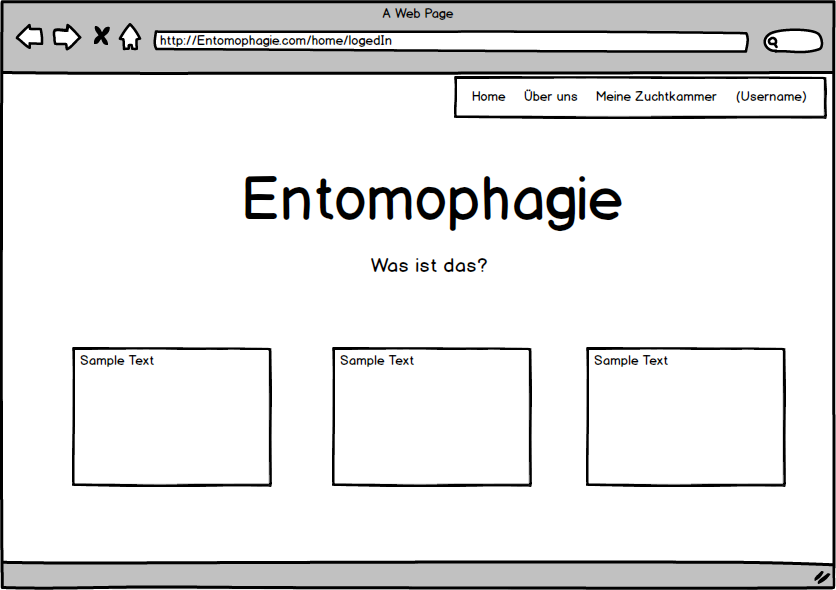
\includegraphics[height=10cm]{figures/Logedin}
Hier sieht man die Ansicht wenn man auf unserer Website Angemeldet ist. Man kann auf seine eigene Zuchtkammer zugreifen indem man auf den Button "Meine Zuchtkammer" klickt und dort die Daten auslesen.
\newpage
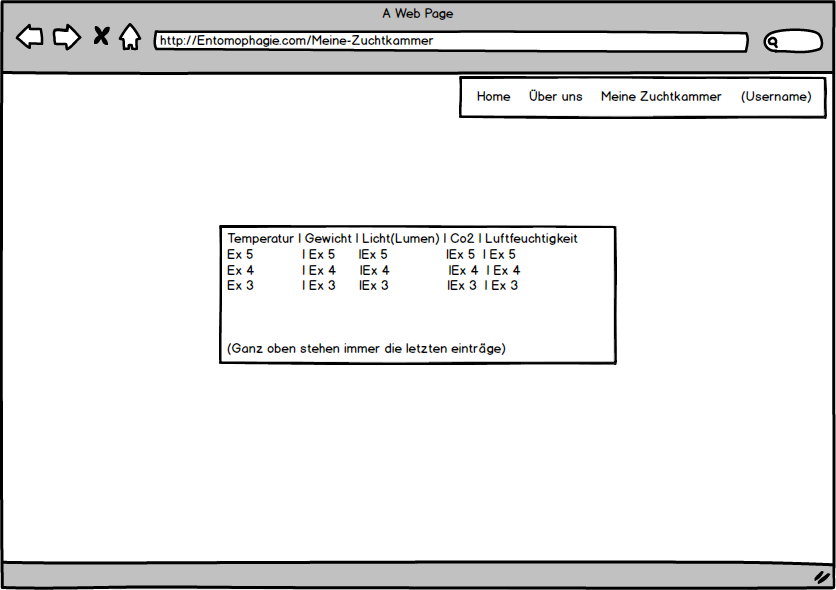
\includegraphics[height=10cm]{figures/Meine-Zuchtkammer}
Auf der Seite "Meine Zuchtkammer" sieht die letzten 10 Daten die meine Zuchtkammer wiedergegeben hat. Diese sind in Absteigender Reihenfolge geordnet,dass heißt, dass der letzte Eintrag ganz oben steht.
\newpage
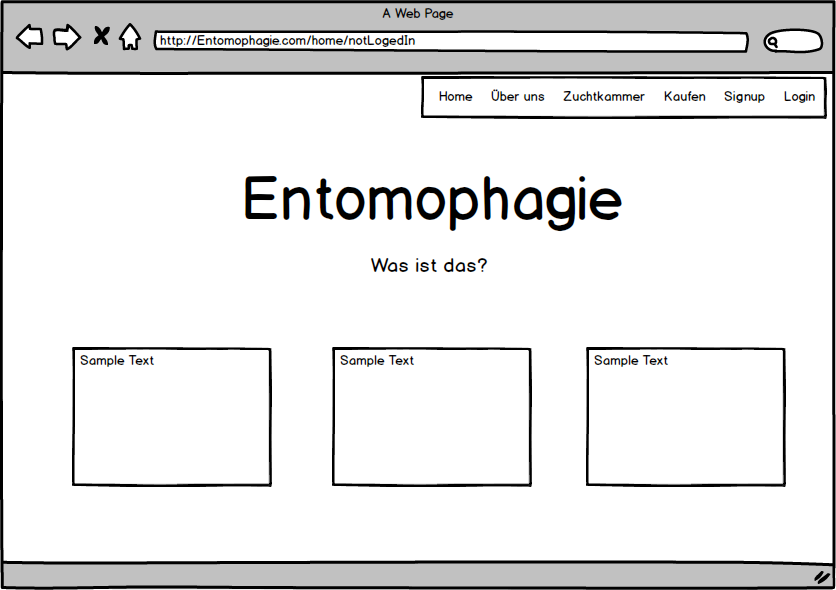
\includegraphics[height=10cm]{figures/NotlogedIN}
Hier Sieht man die Ansicht wenn man auf unserer Website nicht Angemeldet ist. Man kann über den Button "Zuchtkammer" mehr über unsere Zuchtkammern herausfinden, weiter kann man über den Button "Kaufen" seine eigene Zuchtkammer kaufen. Bei Signup kann man sich als neuer Benutzer registrieren, um sich allerdings zu registrieren brauch man zuerst eine Seriennummer die man beim kauf einer Zuchtkammer erhält.
\newpage

\subsection{Datenbankzugriffe}
Unserer Datenbank zugriffe werden von unserem Framework verarbeite, dabei verwendet das Framework CRUD befehle und nach dem MVC Muster. Das heißt es gibt ein unterliegendes Modell welches Daten unserem Controller mitgibt welche wiederum die View erzeugt.

Der gesamte Datenbankzugriff kann mittels Yii2 sehr einfach erstellt werden. Mehr dazu siehe \nameref{sec:gii}

\subsection{Datenübermittlung} \label{sec:daten}

Um die Daten von unsrem Arduino an unsere Datenbank zu senden werden wir in den Brutkasten ein WLAN Modul einbauen und die Daten alle 5-10 Minuten als JSON-Format an unsere REST-Schnittstelle unserer Webapp senden. Das hat den Vorteil das unsere Daten direkt von unserem Brutkasten an die Datenbank gegeben werden kann.
\newline
Für diese Lösung brauchen wir eine REST Schnittelle in unserer Webapp. Dies kann über YII2 sehr einfach realisiert werden. Yii2 hat eine vor implementierte REST Schnittelle welche man nur noch aktivieren muss. Die Daten werden aus der Modell Klasse ausgelesen und über den Controller an die REST-View weitergeleitet. Die ganze Implementierung sind 5-10 Zeilen Code. Die Code Sequenz sehen sie im Kapitel \nameref{sec:Rest}.

\subsection{Rest Schnittelle} \label{sec:Rest}	
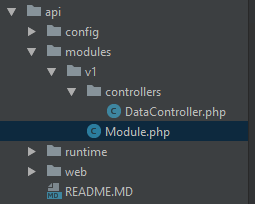
\includegraphics{figures/Ordner}
\newline
Hier sieht man die Ordnerstruktur. Wir erstellen im Obersten Verzeichnis einen neuen Ordner namens 'api' um im Web über folgende URL:'www.entomophagie/api/web/v1/datas' auf unsere Restschnittelle Zugreifen können. Dabei müssen wir darauf achten das wir Groß- und Kleinschreibung beachten. Um dieses Problem zu lösen ist es am einfachsten alle Ordner in unserem Verzeichnis immer klein zuschreiben.\newline
Weiters Kopieren wir 'web', 'config' und den 'runtime' Ordner aus unserem Front- bzw. Backend Ordner. 
\newline
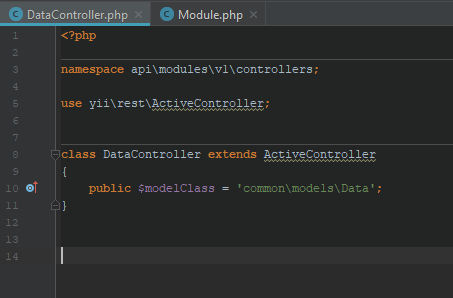
\includegraphics{figures/Controller}
\newline
Hier sieht man die Controller Klasse. In der Controller Klasse müssen wir den Yii eigenen ActiveController einbinden und die Modell Klasse festlegen welche die Daten ausliest.
\newline
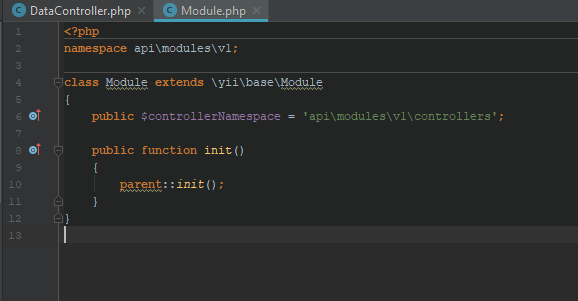
\includegraphics{figures/Modul}
\newline
Hier sieht man die Module Klasse. In der Module Klasse wird unser neuer Rest Controller initialisiert, damit unsere Anwendung diese Verwenden kann. Dort müssen wir unseren Controller den wir zuvor erstellt haben festlegen.
\newline
Wir haben den Rest Controller mit folgendem Online Tutorial erstellt \cite{Restt}.

